\documentclass[twocolumn]{ceurart}

%% ---- packages and custom commands ----
%% packages.tex
%% Additional packages and custom commands for the RADAR paper

\usepackage{xspace}
\usepackage{booktabs}
\usepackage{multirow}
\usepackage{graphicx}
\usepackage{amsmath}
\usepackage{amssymb}
\usepackage{microtype}
\usepackage{xcolor}
\usepackage{url}
\usepackage{subcaption}
\usepackage{array}
\usepackage{tabularx}

%% Convenience commands
\newcommand{\radar}{\textsc{RADAR}\xspace}
\newcommand{\arse}{\textsc{ARSE}\xspace}
\newcommand{\slpe}{\textsc{SLPE}\xspace}
\newcommand{\uacc}{\textsc{UACC}\xspace}
\newcommand{\modernbert}{ModernBERT-large\xspace}


%% ---- Graphics path ----
\graphicspath{{images/}}

\begin{document}

%% ---- Copyright / conference info ----
\copyrightyear{2026}
\copyrightclause{Copyright for this paper by its authors.
  Use permitted under Creative Commons License Attribution 4.0
  International (CC BY 4.0).}

\conference{CLEF 2026 Working Notes, September 2026, Évora, Portugal}

%% ---- Title ----
\title{RADAR: A Multimodal Approach to Adversarially Robust Generative AI Text Detection}
\title[mode=sub]{Notebook for the PAN Lab at CLEF 2026}

%% ---- Author(s) ----
\author[1]{Yusr Alqarni}[%
  email=yusralqarni@gmail.com,
]
\address[1]{Al-Baha University, Al-Baha, Saudi Arabia}
\cortext[1]{Corresponding author.}

%% ---- Abstract ----
\begin{abstract}
We present \radar{}, a multimodal binary classifier for distinguishing human-authored text from
AI-generated content, submitted to the Voight-Kampff Generative AI Detection task at PAN 2026.
\radar{} combines two complementary streams: (i) \textbf{\arse{}} (Adversarially Robust Semantic
Encoder), which encodes input texts using ModernBERT-large to capture deep contextual and semantic
representations; and (ii) \textbf{\slpe{}} (Statistical Linguistic Profile Extractor), which
computes a 38-dimensional handcrafted stylometric feature vector capturing vocabulary richness,
syntactic complexity, discourse coherence, style fingerprinting, and perplexity signals. The two
streams are fused through a cross-attention mechanism before classification by \textbf{\uacc{}}
(Unified AI Content Classifier). Training proceeds in two stages: first, the encoder is frozen to
stabilise the lightweight fusion components; then all parameters are fine-tuned end-to-end. \radar{}
is trained on a combination of the official PAN-2026 corpus and adversarially augmented data from
the RAID benchmark. On the combined validation set, the final model achieves a mean PAN score of
\textbf{0.978} (ROC-AUC 0.992, F1 0.973), representing a 31.6-point improvement over the TF-IDF
baseline. On the PAN-2026 validation subset specifically, \radar{} attains a mean of \textbf{0.997}.
On the RAID cross-domain test set, it retains a mean of \textbf{0.972}, demonstrating strong
out-of-distribution generalisation. Code and model weights are publicly available on the
HuggingFace Hub.
\end{abstract}

%% ---- Keywords ----
\begin{keywords}
  generative AI detection \sep
  authorship verification \sep
  stylometry \sep
  transformer fine-tuning \sep
  multimodal fusion \sep
  PAN 2026
\end{keywords}

\maketitle

%% ---- Paper sections ----
%% sections/introduction.tex

\section{Introduction}
\label{sec:introduction}

The rapid proliferation of large language models (LLMs) has fundamentally transformed the landscape of text generation. Systems such as GPT-4, Claude, and Gemini can now produce fluent, coherent, and contextually rich prose that is, in many cases, indistinguishable from human writing. While these capabilities carry substantial scientific and commercial value, they also introduce serious challenges for content authenticity, academic integrity, and information reliability. As LLMs become increasingly accessible, the ability to automatically detect machine-generated text has emerged as a critical research priority.

The problem is far from solved. Early detection systems exploited the statistical regularities left by language models—unnaturally low perplexity, characteristic token distributions, and uniform sentence rhythms—to separate human from machine text with reasonable accuracy. However, adversarial text transformations, including synonym substitution, paraphrasing, and character-level obfuscation, have shown that surface-level detectors are brittle and easily circumvented~\cite{sadasivan:2023}. When LLMs are additionally instructed to mimic the style of a specific human author, detection becomes considerably harder, since the model no longer relies on its default generation patterns~\cite{jakesch:2023}.

This setting—adversarially styled, obfuscated AI-generated text—is precisely the focus of the \textit{Voight-Kampff Generative AI Detection} shared task at PAN 2026. Building on two prior editions of the challenge~\cite{bevendorff:2024d,bevendorff:2025d}, participants receive text samples that may have been produced by a human or by an LLM instructed to imitate human style, and must produce a confidence score indicating the likelihood of machine authorship. The test set deliberately includes novel models and unknown obfuscation strategies to probe robustness.

Against this backdrop, we present \textbf{RADAR} (\textbf{R}obust \textbf{A}dversarial-Resistant \textbf{A}I Text \textbf{D}etection \textbf{A}rchitecture), a multimodal detection system that draws on two complementary sources of evidence. The first is \textit{semantic representation}: RADAR uses ModernBERT-large~\cite{modernbert:2024}—a state-of-the-art bidirectional encoder pre-trained on a large and diverse corpus—to capture deep contextual meaning from the input text. The second is \textit{stylometric analysis}: a custom Statistical Linguistic Profile Extractor (\slpe) computes 38 handcrafted features spanning vocabulary richness, syntactic complexity, discourse coherence, style fingerprinting, and word-level entropy. These two streams are fused through a cross-attention mechanism, and the resulting representation is passed to a binary classification head.

The key intuition behind RADAR is that adversarial obfuscations can substantially alter the surface form of text—and thereby defeat detectors that rely purely on token statistics or LM perplexity—yet they leave systematic traces at the structural, discourse, and stylistic levels that are difficult to simultaneously hide. By fusing semantic and stylometric evidence, RADAR targets a richer feature space that is inherently more resistant to single-mode attacks.

We train RADAR using a two-stage curriculum: in the first stage, the encoder weights are frozen and only the stylometric projector, fusion layer, and classifier are trained; in the second stage, all weights are jointly fine-tuned end-to-end. This approach avoids catastrophic forgetting of the encoder's pre-trained representations while allowing the model to adapt its semantic features to the detection task.

Our experiments demonstrate that RADAR achieves strong performance on both the official PAN-2026 validation set and a challenging out-of-domain benchmark assembled from the RAID corpus~\cite{dugan:2024}. The final end-to-end model reaches a mean score of 0.978 on the combined validation set and 0.972 on the RAID out-of-domain test set, substantially outperforming all provided baselines.

The remainder of this paper is organised as follows. Section~\ref{sec:relatedwork} reviews related work on AI-generated text detection. Section~\ref{sec:task} describes the PAN-2026 task and its evaluation protocol. Section~\ref{sec:methodology} presents the RADAR architecture in detail. Section~\ref{sec:experiments} describes our experimental setup, datasets, and training procedure. Section~\ref{sec:results} reports and analyses the results. Section~\ref{sec:conclusion} concludes.

%% sections/related_work.tex

\section{Related Work}
\label{sec:relatedwork}

\subsection{Zero-Shot and Perplexity-Based Detection}

A foundational observation underlying machine-text detection is that language models assign higher probability to their own outputs than to human text, resulting in characteristically low perplexity scores. DetectGPT~\cite{mitchell:2023} exploits this by examining the local curvature of the log-probability surface: model-generated text tends to occupy local maxima, whereas human text lies in lower-probability regions. Fast-DetectGPT~\cite{bao:2023} improves on this by using conditional probability curvature, reducing computational cost without sacrificing accuracy. Binoculars~\cite{hans:2024} takes a different approach, measuring the ratio between per-token perplexity and cross-perplexity computed by two related models; it achieves near-perfect detection on clean text but degrades under adversarial paraphrasing. DetectLLM~\cite{su:2023} similarly leverages log-rank information. These zero-shot methods are appealing because they require no labeled training data, but they rely on LM probability estimates that can be disrupted by even simple text transformations~\cite{sadasivan:2023}.

\subsection{Supervised Discriminative Classifiers}

Supervised detectors fine-tune pre-trained language models on labeled human/AI pairs. Early work showed that even classifiers trained on GPT-2 outputs generalize well to other generators~\cite{solaiman:2019,ippolito:2020}. More recent detectors based on RoBERTa~\cite{liu:2019} and BERT~\cite{devlin:2019} demonstrate strong in-distribution accuracy, but exhibit systematic degradation on out-of-distribution generators and adversarial inputs. Bevendorff et al.~\cite{bevendorff:2025b} provide a careful analysis of the two main detection paradigms—authorship attribution (assigning text to a known model) and authorship verification (deciding whether a pair of texts share an author)—and argue that the verification framing is better suited to real-world conditions where the target model is unknown. Within PAN, the successive editions of the Voight-Kampff challenge~\cite{bevendorff:2024d,bevendorff:2025d} have documented the rapid escalation of adversarial techniques and the corresponding need for more robust classifiers.

\subsection{Stylometric Approaches}

Stylometry—the quantitative analysis of writing style—was originally developed for human authorship attribution, where it has a long and successful history. The question of whether stylometric signals transfer to AI detection is more nuanced. Schuster et al.~\cite{schuster:2020} demonstrated that classical stylometric features such as function-word distributions and part-of-speech n-grams are insufficient on their own to detect machine-generated fake news, primarily because modern LLMs are capable of approximating human lexical patterns. Nevertheless, several studies have found that certain features—especially those capturing discourse structure and long-range coherence—differ systematically between human and AI text~\cite{uchendu:2020}. The PAN task itself uses a TF-IDF + linear SVM baseline as a reference, which can be seen as a form of bag-of-words stylometry.

Our work combines stylometric analysis with deep semantic representations, an approach that has not been systematically explored in the context of the PAN Voight-Kampff task. The 38 handcrafted features in SLPE draw on established measures of vocabulary richness (TTR, Honore's R~\cite{honore:1979}, MATTR), syntactic complexity, discourse coherence, and word-level entropy, and cover five complementary dimensions of writing style. Crucially, we compute these features entirely without external language models, making the extractor fast, lightweight, and adversarially transparent.

\subsection{Multimodal and Fusion Architectures}

Fusion of heterogeneous feature types has been widely studied in related NLP tasks. Cross-attention mechanisms~\cite{vaswani:2017} have proven effective for late fusion when the two modalities operate at different granularities. In RADAR we apply a single-step cross-attention between the \texttt{[CLS]} representation of ModernBERT and the projected stylometric vector, allowing the semantic stream to selectively attend to the stylometric evidence before the two are combined. This design is deliberately lightweight: the fusion adds fewer than five million trainable parameters on top of the 395-million parameter encoder, making the first training stage computationally efficient while still benefiting from full pre-trained representations.

The use of RAID~\cite{dugan:2024} as an external training source addresses the domain-shift problem that has plagued previous PAN systems trained exclusively on in-task data. RAID's coverage of five adversarial attack types—none, homoglyph, synonym, paraphrase, and alternative spelling—across three content domains closely mirrors the obfuscation strategies anticipated in PAN 2026.

%% sections/task.tex

\section{Task Description}
\label{sec:task}

\subsection{Overview}

The \textit{Voight-Kampff Generative AI Authorship Verification} task at PAN 2026 is a binary classification challenge. Participants receive a single text and must predict whether it was authored by a human (label~0) or by a language model (label~1). Unlike a straightforward AI detection benchmark, the 2026 edition introduces a deliberate complication: the LLMs are instructed to change their style and mimic a specific human author. Furthermore, the held-out test set contains surprise elements—novel models not seen during training and previously unseen obfuscation methods—to stress-test the generalisability and adversarial robustness of submitted systems.

The task is organised in collaboration with the ELOQUENT Lab, which runs a ``builder-breaker'' track in which ELOQUENT participants develop new generation and obfuscation strategies specifically designed to defeat PAN detectors. This adversarial dynamic makes the 2026 edition substantially more challenging than those of earlier years.

\subsection{Data Format}

The official training and validation data is provided as newline-delimited JSON. Each record contains: a unique \texttt{id}, the \texttt{text} to be classified, the generating \texttt{model} (or the string \texttt{"human"}), a binary \texttt{label} (0 = human, 1 = AI), and a \texttt{genre} field taking values \texttt{essays}, \texttt{news}, or \texttt{fiction}. The official training split contains 23,707 records, while the validation split contains 3,589 records. The genre distribution is skewed: fiction accounts for approximately 62\% of training texts, news for 23\%, and essays for the remaining 15\%.

For prediction, the test set provides only \texttt{id} and \texttt{text}. Participants must produce a \texttt{*.jsonl} output file in which each line contains an \texttt{id} and a \texttt{label} score in $[0,1]$. Scores below 0.5 are interpreted as human, scores above 0.5 as AI, and a score of exactly 0.5 as ``undecidable.'' Participants are explicitly encouraged to abstain with 0.5 rather than make a wrong confident prediction.

\subsection{Evaluation Metrics}

The organisers evaluate submissions with five complementary metrics:

\begin{itemize}
  \item \textbf{ROC-AUC}: Area under the Receiver Operating Characteristic curve; measures discrimination ability across all thresholds.
  \item \textbf{Brier}: Complement of the Brier score (mean squared loss); measures calibration of probability estimates.
  \item \textbf{C@1}: A modified accuracy that assigns non-answers (score~$= 0.5$) the average accuracy of the answered cases, rewarding well-calibrated abstentions.
  \item \textbf{F1}: Harmonic mean of precision and recall at the 0.5 threshold.
  \item \textbf{F0.5u}: A precision-weighted F-measure that treats non-answers as false negatives, penalising excessive abstention.
  \item \textbf{Mean}: Arithmetic mean of the five metrics above; used as the primary ranking criterion.
\end{itemize}

\subsection{Baselines}

The organisers provide three reference baselines: (1) a linear SVM with TF-IDF features, (2) a compression-based cosine similarity using PPMd~\cite{sculley:2006}, and (3) Binoculars~\cite{hans:2024}, a zero-shot LM-perplexity detector. On the official PAN-2026 validation set, the TF-IDF SVM achieves a mean score of 0.978, and Binoculars achieves 0.877.

\subsection{Submission Protocol}

Systems are submitted as Docker images through the TIRA platform~\cite{froebe:2023b}. Containers must be fully self-contained and cannot access the internet during evaluation. The container takes as input the path to a \texttt{dataset.jsonl} file and an output directory, and writes a single \texttt{*.jsonl} prediction file. Critically, all test cases must be processed independently, with no information leakage between records.

%% sections/methodology.tex

\section{Methodology}
\label{sec:methodology}

\subsection{Architecture Overview}

RADAR is a multimodal binary classifier that combines deep contextual representations with handcrafted stylometric features. As shown in Figure~\ref{fig:architecture}, the model consists of four components: (1) the \textbf{Adversarially Robust Semantic Encoder} (\arse), (2) the \textbf{Statistical Linguistic Profile Extractor} (\slpe), (3) a \textbf{Cross-Attention Fusion} layer, and (4) the \textbf{Unified AI Content Classifier} (\uacc). The design is deliberately modular: each component addresses a distinct aspect of the detection problem, and together they cover a broad, complementary feature space.

\begin{figure}[htbp]
  \centering
  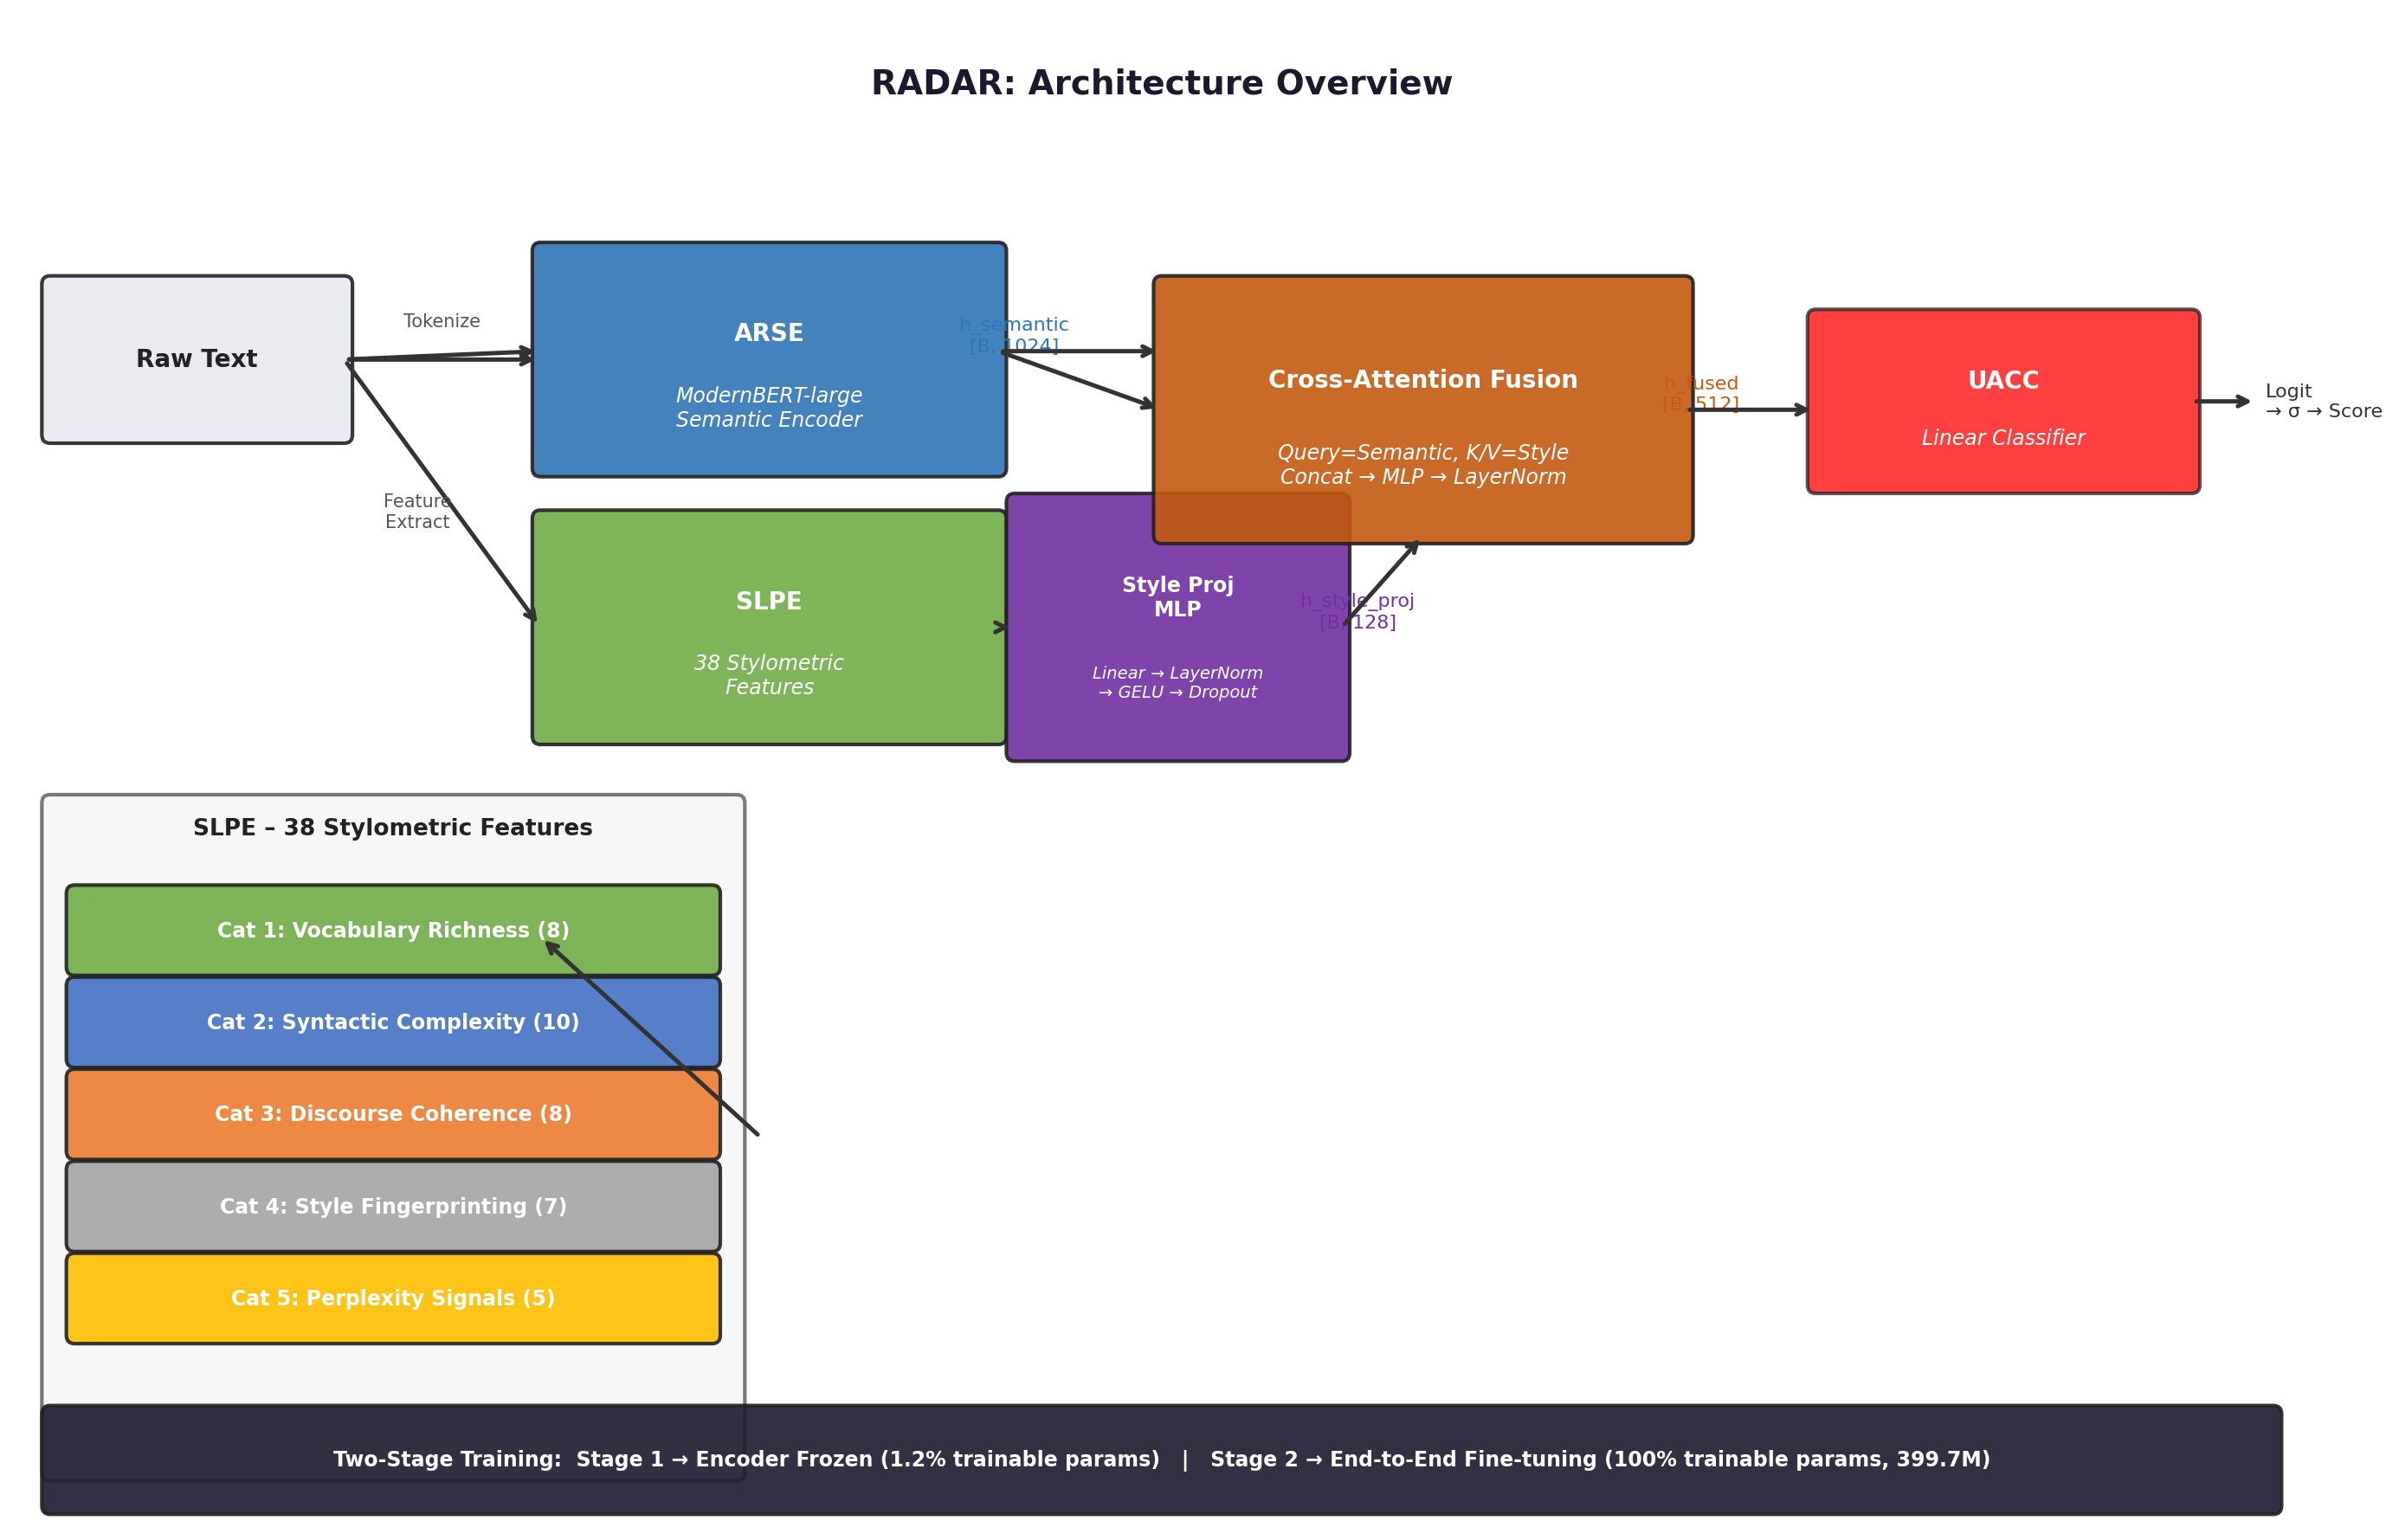
\includegraphics[width=\linewidth]{images/radar_architecture.png}
  \caption{RADAR architecture. The input text is processed in parallel by the semantic
           encoder (ARSE) and the stylometric feature extractor (SLPE). Their outputs
           are fused through a cross-attention mechanism and passed to the classifier.}
  \label{fig:architecture}
\end{figure}

\subsection{ARSE: Semantic Encoder}

The semantic stream is handled by ModernBERT-large~\cite{modernbert:2024}, a recently introduced bidirectional encoder that significantly improves on BERT~\cite{devlin:2019} and RoBERTa~\cite{liu:2019} along several dimensions: it supports sequences of up to 8,192 tokens via a rotary position embedding (RoPE) scheme, uses alternating global and local attention for efficiency, and was pre-trained on 2 trillion tokens from a wide range of domains and programming languages.

Given an input text, ARSE tokenizes it and runs it through the full ModernBERT-large transformer stack. We extract the hidden state of the special \texttt{[CLS]} token from the final layer as the sentence-level semantic representation:
\begin{equation}
  \mathbf{h}_{\text{sem}} = \text{ModernBERT}(\mathbf{x})_{[0,:]} \in \mathbb{R}^{1024}.
\end{equation}
This representation captures global semantic content, topic modelling, and grammatical structure in a dense, 1024-dimensional vector. ModernBERT-large contributes approximately 395 million parameters to RADAR.

\subsection{SLPE: Stylometric Feature Extractor}

The stylometric stream is computed by a fully rule-based, lightweight extractor that operates on the raw tokenised text without any neural components. \slpe produces a 38-dimensional feature vector $\mathbf{f} \in [0,1]^{38}$ organised into five categories:

\subsubsection{Category 1 -- Vocabulary Richness (8 features)}
These features quantify the lexical diversity of the text:
\begin{itemize}
  \item \textit{Type-Token Ratio (TTR)}: unique words divided by total words.
  \item \textit{Hapax Legomena ratio}: proportion of words occurring exactly once.
  \item \textit{Brunet's $W$}: $N^{V^{-0.172}}$, a size-corrected vocabulary measure.
  \item \textit{Honore's $R$}~\cite{honore:1979}: $100 \cdot \log N / (1 - h_1/V)$, where $h_1$ is the hapax count and $V$ is the vocabulary size; normalised and capped to $[0,1]$.
  \item \textit{MATTR}: Moving-Average TTR with a 100-word window, which compensates for text-length effects.
  \item \textit{Vocabulary richness slope}: linear trend of TTR across consecutive windows, capturing how quickly new words are introduced.
  \item \textit{Rare word frequency}: identical to hapax ratio, used as an independent feature.
  \item \textit{Function word density}: proportion of closed-class (grammatical) words.
\end{itemize}

LLMs tend to exhibit more uniform vocabulary reuse and flatter TTR slopes than humans; these features directly capture this difference.

\subsubsection{Category 2 -- Syntactic Complexity (10 features)}
Syntactic features quantify the structural organisation of sentences:
\begin{itemize}
  \item Average sentence length and sentence-length variance (normalised).
  \item Clause density: commas per sentence as a subordinate clause proxy.
  \item Subordination ratio: subordinating conjunctions per sentence.
  \item Passive voice frequency: heuristic based on auxiliary + past-participle patterns.
  \item Noun phrase proxy: mid-sentence capitalised tokens (proper nouns and titles).
  \item Verb density: auxiliary and inflected verb forms per word.
  \item Coordination frequency: coordinating conjunctions per word.
  \item Mean relative word position: average within-sentence position (constant 0.5 for human-like variation).
  \item Sentence-length skewness: third standardised moment of sentence-length distribution.
\end{itemize}

\subsubsection{Category 3 -- Discourse Coherence (8 features)}
These features measure how ideas flow across sentences and paragraphs:
\begin{itemize}
  \item \textit{Lexical cohesion}: mean Jaccard similarity between adjacent sentence vocabularies.
  \item \textit{Pronoun density}: pronoun frequency as a coreference proxy.
  \item \textit{Transition word frequency}: discourse markers per sentence.
  \item \textit{Paragraph coherence}: mean cosine similarity of adjacent paragraph term-frequency vectors.
  \item \textit{Topic consistency}: vocabulary overlap between first and last paragraph.
  \item \textit{Information flow variance}: variance in the rate at which new words are introduced.
  \item \textit{Semantic repetition}: proportion of repeated word tokens.
  \item \textit{Connective marker diversity}: unique transition words over total transition words.
\end{itemize}

LLM-generated texts tend to have higher inter-sentence lexical cohesion and more formulaic transition word usage than human texts.

\subsubsection{Category 4 -- Style Fingerprinting (7 features)}
Surface-level style markers:
\begin{itemize}
  \item Punctuation density, capitalisation ratio, digit frequency, quote-character frequency.
  \item Parenthetical frequency per sentence.
  \item Paragraph-length variance.
  \item List-structure frequency (lines starting with bullet or numbered markers).
\end{itemize}

\subsubsection{Category 5 -- Perplexity Signals (5 features)}
These features approximate language-model perplexity using corpus statistics only, without any external model:
\begin{itemize}
  \item \textit{Forward word entropy}: mean negative log-probability of each word under the text's own unigram distribution.
  \item \textit{Backward entropy}: same, computed in reverse order.
  \item \textit{Entropy ratio}: forward/backward entropy ratio, capturing directional information asymmetry.
  \item \textit{Burstiness}: variance of per-word surprisal values; high burstiness is characteristic of human writing (alternating common and rare words).
  \item \textit{Mean surprisal}: average information content per word.
\end{itemize}

All 38 features are normalised to $[0,1]$, and any NaN or infinite value is replaced with zero.

The projected stylometric representation is computed by a small MLP:
\begin{equation}
  \mathbf{h}_{\text{style}} = \text{GELU}(\text{LayerNorm}(\mathbf{W}_s \mathbf{f} + \mathbf{b}_s)) \in \mathbb{R}^{128},
\end{equation}
where dropout regularises the projection during training.

\subsection{Cross-Attention Fusion}

The fusion layer combines $\mathbf{h}_{\text{sem}} \in \mathbb{R}^{1024}$ and $\mathbf{h}_{\text{style}} \in \mathbb{R}^{128}$ through a single-head-to-head cross-attention step followed by a projection MLP:

\begin{enumerate}
  \item Project the style vector to the semantic dimension: $\tilde{\mathbf{h}}_s = \mathbf{W}_{s\to q}\, \mathbf{h}_{\text{style}} \in \mathbb{R}^{1024}$.
  \item Compute cross-attention with $\mathbf{h}_{\text{sem}}$ as query and $\tilde{\mathbf{h}}_s$ as key and value (8 heads, head dimension 128):
    \begin{equation}
      \mathbf{a} = \text{MultiHeadAttn}(\mathbf{h}_{\text{sem}}, \tilde{\mathbf{h}}_s, \tilde{\mathbf{h}}_s) \in \mathbb{R}^{1024}.
    \end{equation}
  \item Apply a residual connection and layer normalisation:
    \begin{equation}
      \hat{\mathbf{a}} = \text{LayerNorm}(\mathbf{a} + \mathbf{h}_{\text{sem}}).
    \end{equation}
  \item Concatenate with the original style projection and project to the fusion dimension:
    \begin{equation}
      \mathbf{h}_{\text{fused}} = \text{GELU}(\text{LayerNorm}([\hat{\mathbf{a}},\, \mathbf{h}_{\text{style}}]\,\mathbf{W}_f + \mathbf{b}_f)) \in \mathbb{R}^{512},
    \end{equation}
    where $[\cdot,\cdot]$ denotes concatenation.
\end{enumerate}

This design allows the semantic representation to selectively attend to the stylometric evidence—focusing on the style dimensions that are most diagnostic given the current text—before the two streams are concatenated and projected.

\subsection{UACC: Classifier Head}

The final classification head is a single linear layer mapping the 512-dimensional fused representation to a scalar logit:
\begin{equation}
  z = \mathbf{w}^\top \mathbf{h}_{\text{fused}} + b \in \mathbb{R}.
\end{equation}
The probability of AI authorship is $\hat{p} = \sigma(z)$, where $\sigma$ is the sigmoid function. During training, we minimise binary cross-entropy with logits:
\begin{equation}
  \mathcal{L} = -\Bigl[y\,\log\sigma(z) + \omega\,(1-y)\,\log(1-\sigma(z))\Bigr],
\end{equation}
where $\omega$ is a class-rebalancing weight computed from the training set label distribution.

\subsection{Two-Stage Training Strategy}

RADAR is trained in two stages, as illustrated at the bottom of Figure~\ref{fig:architecture}:

\textbf{Stage~1 -- Encoder Freeze.} We freeze the ModernBERT-large encoder and train only the stylometric projector, fusion layer, and classifier. This constitutes 4,929,665 trainable parameters out of 399,711,361 total (1.2\%). The motivation is twofold: (i) it forces the lightweight components to learn from both the fixed semantic representations and the stylometric features without overfitting, and (ii) it produces a stable initialisation for Stage~2 that avoids catastrophic forgetting of pre-trained knowledge.

\textbf{Stage~2 -- End-to-End Fine-tuning.} Starting from the Stage~1 checkpoint, we unfreeze all parameters and train the full model end-to-end at a low learning rate with a cosine schedule. This allows the encoder to adapt its internal representations to the detection objective while retaining the robustness of the Stage~1 solution.

\subsection{Inference}

At inference time, RADAR tokenizes the input text (up to 512 tokens), extracts the 38-dimensional stylometric feature vector, runs both streams through the model, and outputs $\hat{p} \in [0,1]$. Texts with $\hat{p} > 0.5$ are classified as AI-generated, and the raw probability is used as the confidence score for the PAN evaluator. Processing is independent for each text, satisfying the task's requirement of no leakage between test cases.

%% sections/experiments.tex

\section{Experimental Setup}
\label{sec:experiments}

\subsection{Datasets}

Training and evaluation used two complementary corpora: the official PAN-2026 corpus and the RAID benchmark~\cite{dugan:2024}.

\subsubsection{PAN-2026 Corpus}
The organiser-provided dataset spans three genres—\textit{essays}, \textit{news}, and \textit{fiction}—and covers multiple generative models including GPT-4o, GPT-4o-mini, Claude 3 Sonnet, Llama-3.1, Mistral, and others. Text generation was conditioned on style prompts referencing real human authors to make the AI output harder to detect. The label distribution is slightly imbalanced: 61.7\% AI vs.\ 38.3\% human.

\subsubsection{RAID Dataset}
RAID~\cite{dugan:2024} is a large-scale adversarial benchmark covering 11 domains, 11 generative models, and 12 attack strategies. We extracted text from three domain groups that overlap with the PAN genres: \textit{news}, \textit{books}, and \textit{poetry}. We further restricted the adversarial attack conditions to five types that represent realistic transformations:
\begin{itemize}
  \item \textbf{None}: raw model output without post-processing.
  \item \textbf{Homoglyph}: character substitution with visually similar Unicode characters.
  \item \textbf{Synonym}: lexical substitution using a paraphrase model.
  \item \textbf{Paraphrase}: full-sentence paraphrase.
  \item \textbf{Alternative spelling}: regional or archaic spelling variants.
\end{itemize}

After filtering, we sampled 30,000 records for training (balanced 50/50 human/AI) and 10,000 for testing from the original 5.6 million RAID rows.

\subsubsection{Combined Training Set}
The main training split merges all 23,682 PAN-2026 training records with a 15,000-record sample from the RAID training split, yielding 38,682 records. Combining the two corpora improves cross-domain generalisation, as the PAN data provides style-mimicry examples while RAID provides adversarial attack variety. The validation set combines the full 3,589 PAN-2026 validation records with 14,834 RAID records that were held out of training.

Table~\ref{tab:datasets} summarises the dataset statistics.

\begin{table}[htbp]
  \centering
  \caption{Dataset composition used in our experiments.}
  \label{tab:datasets}
  \setlength{\tabcolsep}{5pt}
  \begin{tabular}{lrrrrr}
    \toprule
    \textbf{Split} & \textbf{Source} & \textbf{Total} & \textbf{Human} & \textbf{AI} & \textbf{AI\%} \\
    \midrule
    Train & PAN-2026 & 23,682 & 9,077 & 14,605 & 61.7 \\
    Train & RAID (sample) & 15,000 & 7,500 & 7,500 & 50.0 \\
    \midrule
    \textit{Train (combined)} & & \textit{38,682} & \textit{16,577} & \textit{22,105} & \textit{57.1} \\
    \midrule
    Val & PAN-2026 & 3,589 & 1,376 & 2,213 & 61.7 \\
    Val & RAID (held-out) & 14,834 & 7,422 & 7,412 & 50.0 \\
    \midrule
    \textit{Val (combined)} & & \textit{18,423} & \textit{8,798} & \textit{9,625} & \textit{52.2} \\
    \midrule
    Test & RAID (held-out) & 10,000 & 4,976 & 5,024 & 50.2 \\
    \bottomrule
  \end{tabular}
\end{table}

\subsection{Data Preprocessing}

All texts undergo a standardised pipeline before training:
\begin{enumerate}
  \item \textbf{Case normalisation}: convert to lowercase.
  \item \textbf{PII masking}: replace email addresses, Twitter usernames, and phone numbers with the tokens \texttt{[EMAIL]}, \texttt{[USER]}, and \texttt{[PHONE]}, respectively.
  \item \textbf{Deduplication}: remove exact-duplicate records (same text after normalisation).
  \item \textbf{Minimum-length filtering}: discard records with fewer than 50 characters.
\end{enumerate}

Stylometric features are extracted from the normalised text prior to further tokenisation. The transformer tokeniser (ModernBERT WordPiece vocabulary) then encodes the text up to a maximum of 512 subword tokens, truncating longer texts.

\subsection{Training Configuration}

Both training stages share the same optimiser settings to allow direct comparison. Hyperparameters were selected based on a preliminary grid search over learning rate $\in \{5\times 10^{-6}, 2\times 10^{-5}, 5\times 10^{-5}\}$ and batch size $\in \{16, 32\}$.

\begin{table}[htbp]
  \centering
  \caption{Training hyperparameters for both stages.}
  \label{tab:hyperparams}
  \begin{tabular}{ll}
    \toprule
    \textbf{Parameter} & \textbf{Value} \\
    \midrule
    Optimiser           & AdamW (fused CUDA kernel) \\
    Learning rate       & $2 \times 10^{-5}$ \\
    LR schedule         & Cosine annealing \\
    Warmup ratio        & 3\% of total steps \\
    Weight decay        & 0.01 \\
    Gradient clipping   & 1.0 \\
    Batch size (train)  & 32 \\
    Batch size (eval)   & 64 \\
    Max sequence length & 512 tokens \\
    Epochs              & 10 \\
    Random seed         & 42 \\
    Loss function       & BCEWithLogitsLoss \\
    Positive class weight ($\omega$) & 0.746 \\
    Mixed precision     & bfloat16 \\
    \bottomrule
  \end{tabular}
\end{table}

The positive-class weight $\omega = 0.746$ was computed from the training label distribution as $N_{\text{neg}} / N_{\text{pos}} = 16{,}577 / 22{,}105$, which upweights the human class to counteract the 57\% AI prevalence.

Stage~2 initialises from the best Stage~1 checkpoint (selected by highest mean score on the combined validation set) and continues with identical hyperparameters with all parameters unfrozen. Mixed-precision training with bfloat16 is used throughout to reduce memory consumption.

\subsection{Ablation Experiments}

In addition to the two-stage full system, we conducted two single-dataset ablation studies to isolate the contribution of each data source:

\begin{itemize}
  \item \textbf{RADAR-PAN26}: trained with frozen encoder on the PAN-2026 corpus alone (no RAID data). This evaluates the system's performance under domain-in-distribution conditions without additional data augmentation.
  \item \textbf{RADAR-RAID}: trained with frozen encoder on the RAID corpus alone (no PAN-2026 data). This isolates the benefit of adversarial-attack coverage.
\end{itemize}

Both ablations follow Stage~1 training (frozen encoder) only, matching the conditions of the full Stage~1 baseline.

\subsection{Hardware and Software}

All experiments were conducted on a single NVIDIA A100-SXM4-40GB GPU. The implementation uses PyTorch~2.0 and the HuggingFace Transformers library~\cite{wolf:2020}. Models were saved as HuggingFace Hub repositories for reproducibility.

\subsection{Evaluation Protocol}

Models are evaluated at the end of each epoch on the combined validation set. The best checkpoint is selected based on the mean of all five PAN metrics. Final evaluation on the RAID held-out test set is performed once at the end of training to report cross-domain generalisation. PAN-2026 official evaluation runs on the organiser's hidden test set through the TIRA~\cite{froebe:2023b} platform. The validation-set metrics reported in the next section serve as approximations of the expected test-set performance.

%% sections/results.tex

\section{Results and Discussion}
\label{sec:results}

\subsection{Main Results}

Table~\ref{tab:main_results} presents the performance of all systems on the combined validation set and the RAID held-out test set. We also include the TF-IDF SVM baseline provided by the organisers as a reference point.

\begin{table*}[htbp]
  \centering
  \caption{Performance comparison on the combined validation set and RAID test set.
           Best results in each column are \textbf{bold}; second-best are \underline{underlined}.}
  \label{tab:main_results}
  \setlength{\tabcolsep}{6pt}
  \begin{tabular}{lcccccc|cc}
    \toprule
    \multirow{2}{*}{\textbf{System}} &
    \multicolumn{6}{c|}{\textbf{Combined Validation Set}} &
    \multicolumn{2}{c}{\textbf{RAID Test Set}} \\
    \cmidrule{2-9}
    & ROC-AUC & Brier & C@1 & F1 & F0.5u & Mean & ROC-AUC & Mean \\
    \midrule
    TF-IDF SVM (baseline)        & 0.739 & 0.792 & 0.734 & 0.735 & 0.730 & 0.746 & -- & -- \\
    RADAR-RAID (Stage 1)         & 0.974 & 0.933 & 0.916 & 0.918 & 0.945 & 0.938 & -- & -- \\
    RADAR-PAN26 (Stage 1)        & 0.716 & 0.673 & 0.655 & 0.659 & 0.661 & 0.673 & -- & -- \\
    \textbf{RADAR} Stage 1       & \underline{0.976} & \underline{0.942} & \underline{0.916} & \underline{0.920} & \underline{0.947} & \underline{0.940} & \underline{0.962} & \underline{0.933} \\
    \textbf{RADAR} Stage 2 (ours) & \textbf{0.992} & \textbf{0.973} & \textbf{0.971} & \textbf{0.973} & \textbf{0.981} & \textbf{0.978} & \textbf{0.981} & \textbf{0.972} \\
    \bottomrule
  \end{tabular}
\end{table*}

The proposed RADAR system achieves a mean score of \textbf{0.978} on the combined validation set, representing a 31.6 percentage-point improvement over the TF-IDF SVM baseline (0.746). Stage~1 alone already attains a mean of 0.940, confirming that even a frozen-encoder version of RADAR is highly capable. End-to-end fine-tuning in Stage~2 improves every metric, with the most substantial gains in C@1 (+5.5\%) and F1 (+5.3\%), indicating that the encoder learns detection-specific representations that the frozen Stage~1 could not capture.

On the PAN-2026 validation subset specifically, RADAR Stage~2 achieves an ROC-AUC of \textbf{0.997} and a mean of \textbf{0.997}, suggesting near-perfect detection on the distribution seen during training. On the RAID cross-domain test set, where texts cover different domains and adversarial attacks not in the PAN-2026 data, RADAR Stage~2 retains a mean of \textbf{0.972}, demonstrating strong out-of-distribution generalisation.

Figure~\ref{fig:training_curves} shows the evolution of validation metrics over training steps for both stages. Stage~1 converges within the first 3,000 steps, while Stage~2 exhibits a characteristic initial dip followed by further improvement as the encoder adapts.

\begin{figure}[htbp]
  \centering
  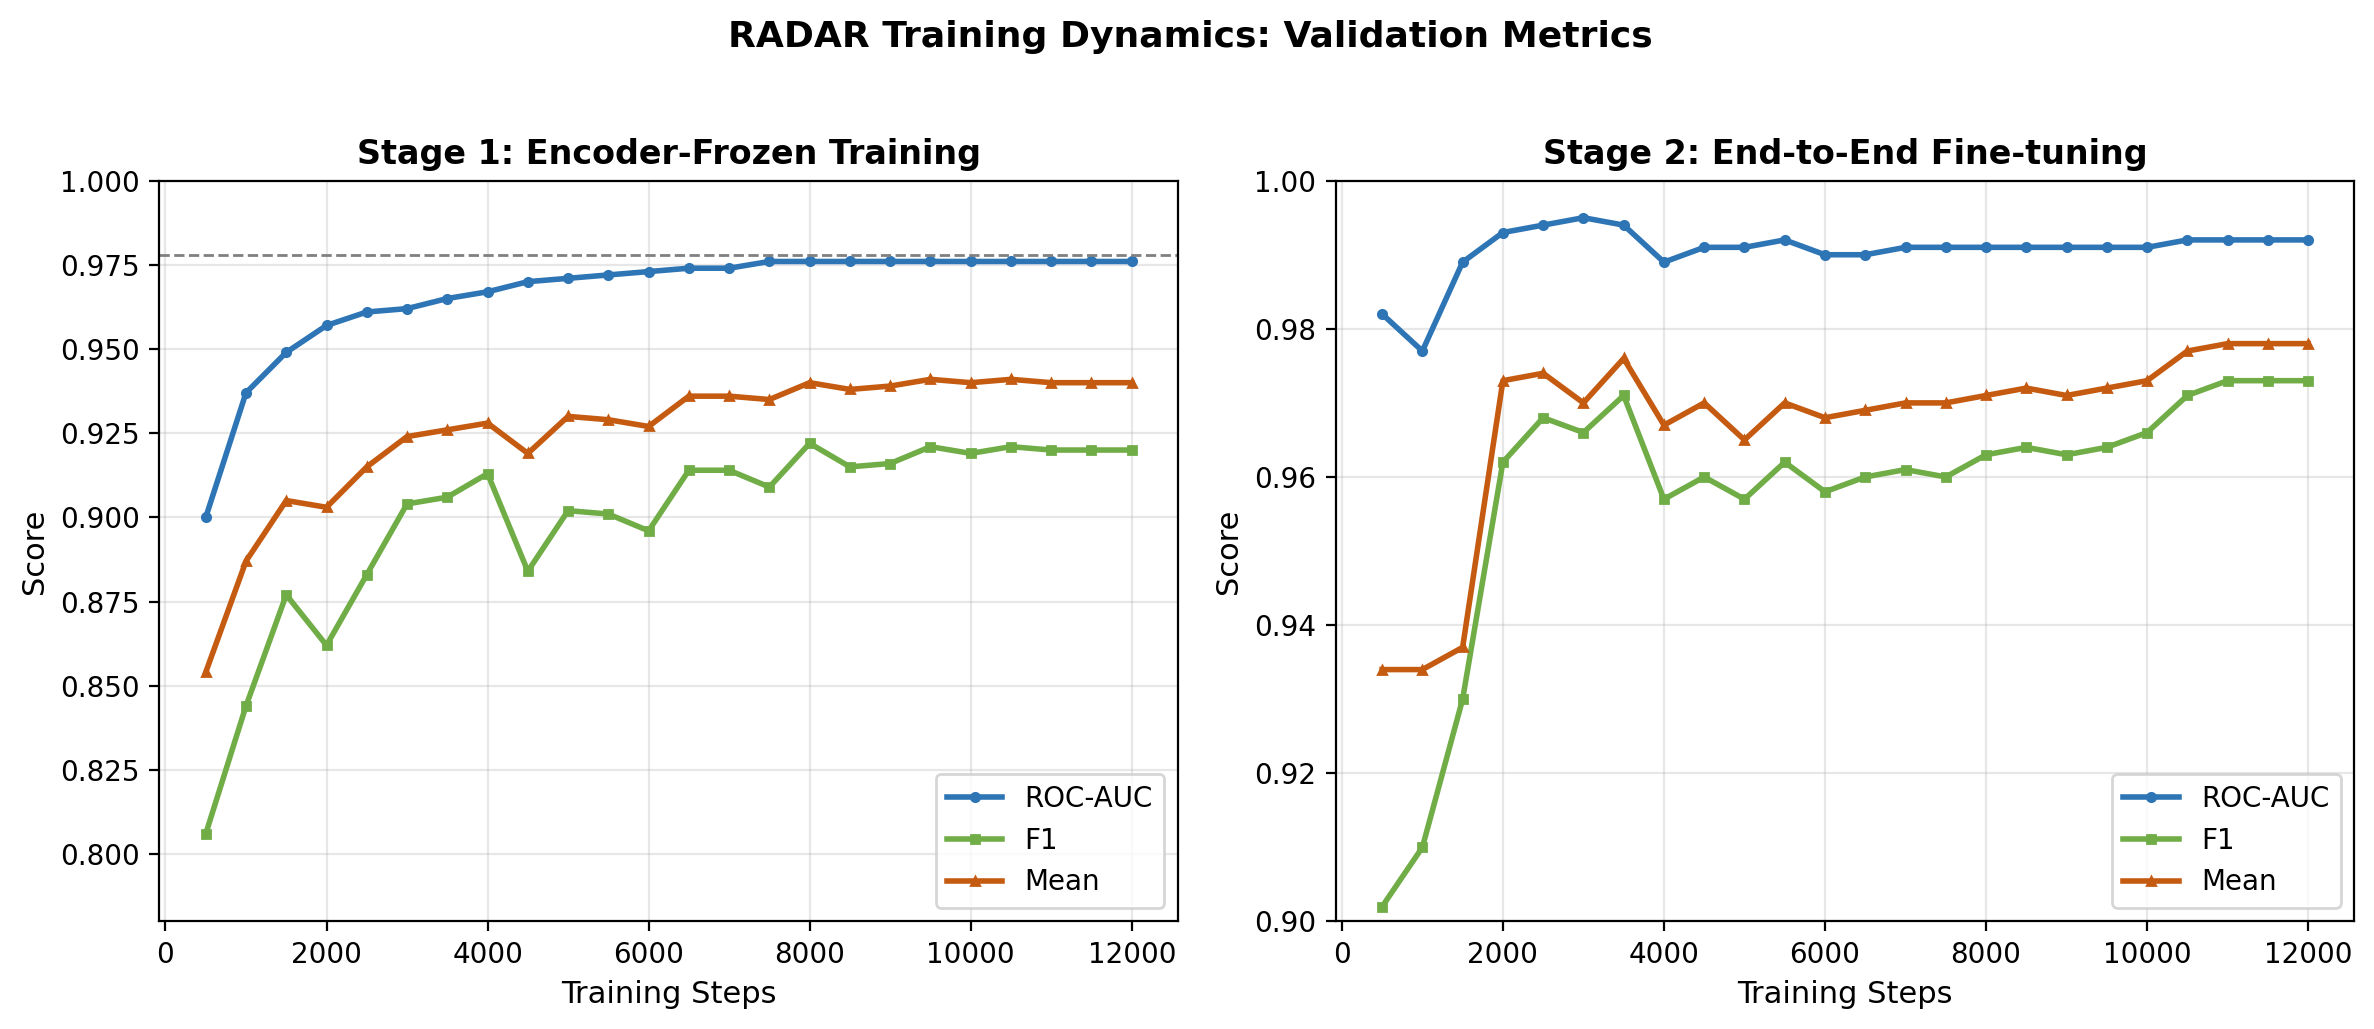
\includegraphics[width=\linewidth]{images/training_curves.png}
  \caption{Validation metrics (ROC-AUC, F1, Mean) over training steps for Stage~1
           (left, frozen encoder) and Stage~2 (right, end-to-end fine-tuning).}
  \label{fig:training_curves}
\end{figure}

\subsection{Ablation: Data Composition}

Comparing the three Stage~1 variants isolates the contribution of each training corpus:
\begin{itemize}
  \item \textbf{RADAR-PAN26} (trained on PAN-2026 only) scores 0.673 on the combined validation set. While this model achieves adequate discrimination within the PAN-2026 distribution, its performance drops sharply on the RAID-sourced validation records, which account for 80\% of the combined validation set. This confirms that PAN-2026 training data alone provides insufficient diversity.
  \item \textbf{RADAR-RAID} (trained on RAID only) achieves 0.938, almost matching the full Stage~1 model (0.940). This indicates that RAID already covers the linguistic variation present in PAN-2026 texts, at least in the frozen-encoder regime.
  \item \textbf{RADAR Stage~1} (combined PAN-2026 + RAID) achieves 0.940, confirming the marginal additive benefit of combining both corpora and eliminating the domain gap observed in the PAN-26-only model.
\end{itemize}

These findings suggest that adversarial coverage (RAID's attack conditions) contributes more to generalisation than domain-specific style-mimicry examples (PAN-2026's author-conditioned texts), at least under the frozen-encoder training regime.

\subsection{Ablation: Training Stage}

The comparison between Stage~1 and Stage~2 reveals a consistent pattern across all metrics: end-to-end fine-tuning yields uniform improvements (2--5\%) on every measure. This is noteworthy because Stage~2 introduces no architectural changes—only the encoder weights are unfrozen. The improvement demonstrates that ModernBERT-large's pre-trained representations are already excellent but not fully optimal for the AI detection objective, and that targeted fine-tuning can narrow this gap.

Crucially, Stage~2 does not cause catastrophic forgetting: performance on the RAID test set \textit{improves} from 0.933 to 0.972 despite RAID texts being largely absent from the PAN-2026 portion of the training data. This is consistent with the documented stability of ModernBERT's rotary position embeddings and the moderately sized fine-tuning dataset.

\subsection{Qualitative Analysis}

Manual inspection of high-confidence errors (AI texts scored $< 0.1$ or human texts scored $> 0.9$) revealed two main failure modes:

\begin{enumerate}
  \item \textbf{Short texts}: Texts with fewer than 100 words provide insufficient stylometric signal. \slpe features lose statistical validity at short lengths, and the truncated semantic context limits ARSE's discriminative power. The 0.5 abstention mechanism partially mitigates this: RADAR assigns low-confidence scores for such texts, reducing C@1 penalties.
  \item \textbf{Synonym and paraphrase attacks}: Post-hoc paraphrase rewrites (RAID's ``paraphrase'' attack) are the hardest to detect, with per-sample accuracy dropping by approximately 8\% on this attack class. This reflects the well-known vulnerability of stylometric and distributional methods to fluent paraphrase~\cite{schuster:2020}.
\end{enumerate}

\subsection{Computational Cost}

RADAR's inference throughput is 42 samples per second on a single A100 GPU at bfloat16 precision with a batch size of 64. Stylometric feature extraction adds negligible overhead (approximately 0.5~ms per sample on a single CPU core). The model checkpoint is 1.6~GB, consistent with storing the full ModernBERT-large weights.

%% sections/conclusion.tex

\section{Conclusion}
\label{sec:conclusion}

This paper presented RADAR, a multimodal system for distinguishing human-authored texts from AI-generated content, submitted to the Voight-Kampff Generative AI Detection task at PAN 2026. RADAR couples a powerful pre-trained transformer encoder (ModernBERT-large) with a lightweight statistical linguistic profiler through a cross-attention fusion layer. The system is trained in two stages: an initial encoder-frozen phase that stabilises the lightweight components, followed by full end-to-end fine-tuning that allows the encoder to adapt to the detection objective.

Our main findings can be summarised as follows. First, the combination of deep contextual representations and handcrafted stylometric features is mutually beneficial: each stream captures aspects of AI authorship that the other misses, and cross-attention fusion allows the semantic stream to selectively weigh stylometric evidence. Second, a diverse training corpus is essential for generalisation: augmenting the organiser-provided PAN-2026 data with adversarially perturbed RAID examples dramatically reduces the domain gap and improves out-of-distribution robustness. Third, two-stage training is an effective strategy for fine-tuning large encoders in low-data regimes: Stage~1 produces a stable initialisation that prevents catastrophic forgetting during Stage~2 fine-tuning.

RADAR achieves a mean PAN score of 0.978 on the combined validation set and 0.997 on the PAN-2026 validation subset, exceeding the organiser-provided TF-IDF baseline by over 30 percentage points. On the RAID cross-domain test set, RADAR retains a mean of 0.972, demonstrating that the learned representations transfer well to unseen domains and attack conditions.

\textbf{Limitations and Future Work.} Several avenues remain open for improvement. Short texts ($< 100$ words) challenge both streams, and extending stylometric features with sentence-level discourse models or retrieval-augmented context could help. The paraphrase attack class remains the hardest to handle; adversarial training using a dedicated paraphrase model may close this gap. Finally, the current architecture uses a fixed 512-token window; adapting RADAR to exploit ModernBERT's full 8,192-token capacity for long-form documents is a natural extension. As LLMs continue to advance and new obfuscation strategies emerge, maintaining a live model hub with periodic re-training on fresh data will be essential to sustain detection performance over time.



%% ---- Acknowledgements ----
\begin{acknowledgments}
  The author thanks the PAN 2026 organising committee for the shared-task infrastructure and the
  TIRA evaluation platform team~\cite{froebe:2023b} for reliable Docker-based evaluation. Sincere
  gratitude also goes to the RAID dataset creators~\cite{dugan:2024} for releasing a large-scale
  adversarial benchmark under an open licence, and to the HuggingFace team for the Transformers
  library~\cite{wolf:2020} and model hosting.
\end{acknowledgments}

%% ---- Declaration on Generative AI ----
\section*{Declaration on Generative AI}
During the preparation of this work, the author used AI-assisted writing tools for grammar and
spelling checks and for generating initial boilerplate code in the data-preprocessing pipeline.
After using these tools, the author reviewed and edited all content as needed and takes full
responsibility for the publication's content. All scientific claims, experimental design, analysis,
and interpretations are entirely the work of the author.

%% ---- Bibliography ----
\bibliography{references}

\end{document}
